\documentclass[12pt,letterpaper]{article}
\usepackage[utf8]{inputenx} %Codificacion del texto (ISO Latin1 encoding)

\usepackage{fancyhdr} %Permite acomodar a tu gusto la parte de arriba y
% abajo del documento
\usepackage[spanish]{babel} %Permite definir el idioma del dcumento
\usepackage{graphicx} %Permite exportar imagenes en formato eps
\usepackage{url} %Tipo de fuente para correos y paginas
\usepackage{pgf}
\usepackage{fleqn}
\usepackage{amssymb}
\usepackage{amsmath}
\usepackage{fancyvrb}
\usepackage{makeidx}
\usepackage{colortbl} %Permite colocar colores a las tablas
\usepackage{multirow}
\usepackage{booktabs}
\usepackage{moreverb}
\usepackage{rotating}
\usepackage{lastpage}
\usepackage[final]{pdfpages}
%%%%%%%%%%
%Margenes%
%%%%%%%%%%
\usepackage[top=3cm,bottom=3cm,left=3.5cm,right=3.5cm,footskip=1.5cm,headheight=1.5cm,headsep=.5cm,textheight=3cm]{geometry}
%%%%%%%%%%%%%%%%%%%%%%
%Estilo del documento%
%%%%%%%%%%%%%%%%%%%%%%
\pagestyle{fancyplain}

%%%%%%%%%%%%%%%%%%%%%%%%%%%%%%%%%%%%%%%%%%%
%Fancyheadings. Top y Bottom del documento%
%%%%%%%%%%%%%%%%%%%%%%%%%%%%%%%%%%%%%%%%%%%
% Recuerde que en este documento la portada del documento no posee
% numeracion, pero de igual manera llamaremos a esa primera pagina la numero
% 1, y la que viene la dos. Esto es para tener una idea de las que
% llamaremos pares e impares
\lhead{Laboratorio mat023} %Parte superior izquierda
\rhead{\bf \it Preinforme 2} %Parte superior derecha
\lfoot{\it Victor Gonzalez} %Parte inferior izquierda. \thepage indica
% el numero de pagina
\cfoot{\bf \thepage} %Parte inferior central
\rfoot{página \thepage\ de \pageref{LastPage}} %Parte inferior derecha
\renewcommand{\footrulewidth}{0.4pt} %Linea de separacion inferior

\begin{document}
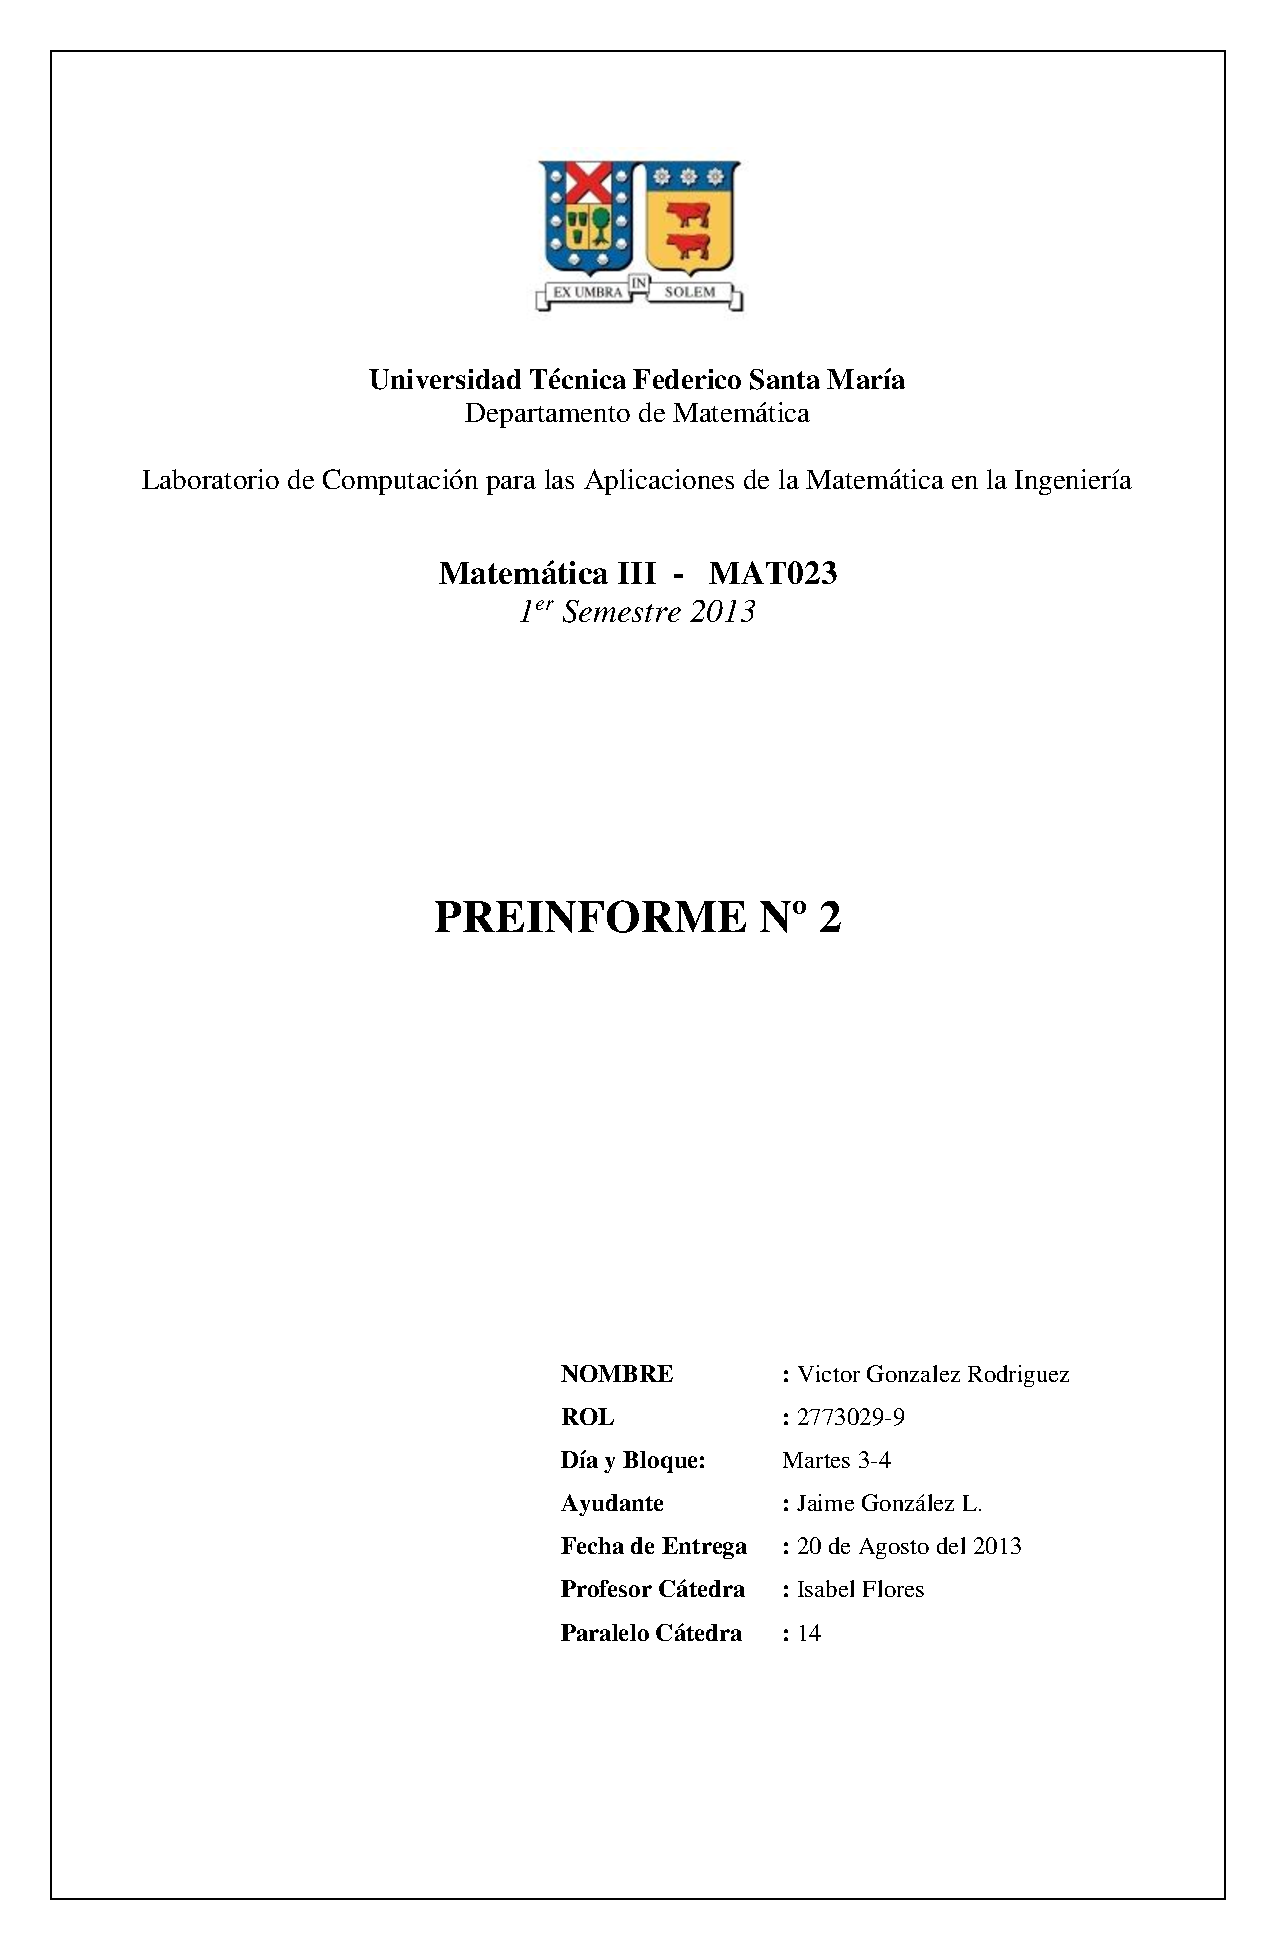
\includepdf[pages={1}]{Portada_Mat023_2013_1.pdf}

\section{Enunciado}
Para los problemas que se entregan a continuación, se deben usar las siguientes constantes:
\begin{description}
\item[$\alpha$] : penúltimo dígito no nulo de su rol. En mi caso: $9$.
\item[$\beta$] : su bloque horario. En mi caso: $2$. 
\end{description}

Usando \textbf{Transformada de Laplace}, resolver el sistema de ecuaciones diferenciales de coeficientes constantes.

\begin{center}
	\begin{tabular}{ p{3.5cm} |}
	$\dfrac{dx}{dt} = \alpha x + \beta y$ \\
	\smallskip \\
	$\dfrac{dy}{dt} = -\beta x + \alpha y$ \\
	\smallskip \\
	\hline
	\end{tabular}
\end{center}

Donde $x(0)=\beta$, $y(0)=\alpha$

\section{Planteo}
Primero, reemplazamos los alfa y beta por los valores respectivos, quedandonos el siguiente sistema:

\begin{equation}\dfrac{dx}{dt} = 9 x + 2 y\end{equation}
\begin{equation}\dfrac{dy}{dt} = -2 x + 9 y\end{equation}

Donde $x(0)=2$, $y(0)=9$ \\

Luego, nos encontramos frente a un sistema de ecuaciones diferenciales, al cual se le debe encontrar soluciones empleando \textit{Transformaciones de Laplace}.

El curso a seguir para resolver esto, sigue la misma mecánica que se utiliza para resolver sistemas de ecuaciones normales, pero con algunos pasos extras, ya que la idea es dejar resuelta una incógnita conveniente, para luego encontrar la otra (tal cual como en un sistema normal).

El curso a seguir para resolver una ecuación diferencial utilizando \textit{Transformaciones de Laplace}, es el siguiente:

\begin{enumerate}
	\item Calculamos la transformada de Laplace de una ecuación, para obtener \textit{la ecuación subsidiaria}.
	\item Luego, despejamos la transformada de Laplace de esta ecuación subsidiaria.
	\item Buscamos la función inversa de la transformada que encontramos. Esta inversa de Laplace, es la solución de la ecuación diferencial.
\end{enumerate}


\section{Desarrollo}
Primero alineamos todos los valores de las ecuaciones (1) y (2) hacia la izquierda, y luego aplicamos la transformada de Laplace en ambas ecuaciones:

\begin{equation}\dfrac{dx}{dt} - 9 x - 2 y = 0\end{equation}
\begin{equation}\dfrac{dy}{dt} + 2 x - 9 y = 0\end{equation}

\begin{equation}sX-x(0)-9X-2Y=0\end{equation}
\begin{equation}sY-y(0)+2X-9Y=0\end{equation}

Ya que $x(0)=2$ y $y(0)=9$, las reemplazamos en (5) y (6). Luego, factorizamos y acomodamos:

\begin{equation}(s-9)X-2Y=2\end{equation}
\begin{equation}2X+(s-9)Y=9\end{equation}

Multiplicamos a (7) por $(s-9)$ y a (8) por $2$:

\begin{equation}(s-9)^2 X-2(s-9)Y=2(s-9)\end{equation}
\begin{equation}4X+2(s-9)Y=18\end{equation}

Si sumamos a (9) y (10), obtenemos la siguiente ecuación:

\begin{equation}((s-9)^2+4)X=2s\end{equation}

Simplificando y despejando:

\begin{equation}X(s)=2\dfrac{s}{(s-9)^2+2^2}\end{equation}

Podemos notar que esta transformada de Laplace, tiene un cierto parecido a la transformada del coseno. La cual es:

\begin{center}
	$\mathcal{L}\{cos(at)\} = \dfrac{s}{s^2+a^2}$
\end{center}

Luego, sumamos un \textit{cero} conveniente:

\begin{equation}X(s) = 2\dfrac{s}{(s-9)^2+2^2} = 2\left(\dfrac{s-9}{(s-9)^2+2^2} + \dfrac{9}{(s-9)^2+2^2}\right)\end{equation}
\newpage

Ahora notamos que el lado derecho de la suma, es similar a la transformada de Laplace del seno, el cual es:

\begin{center}
	$\mathcal{L}\{sin(at)\} = \dfrac{a}{s^2+a^2}$
\end{center}

Luego, multiplicamos el lado derecho de la suma, por un \textit{uno} conveniente:

\begin{equation*}X(s) = 2\left(\dfrac{s-9}{(s-9)^2+2^2} + \dfrac{\frac{2}{9}}{\frac{2}{9}}\dfrac{9}{(s-9)^2+2^2}\right)\end{equation*}

\begin{equation*}X(s) = 2\left(\dfrac{s-9}{(s-9)^2+2^2} + \dfrac{9}{2}\dfrac{2}{(s-9)^2+2^2}\right) \end{equation*}

\begin{equation}X(s) = \dfrac{2(s-9)}{(s-9)^2+2^2} + 9\dfrac{2}{(s-9)^2+2^2} \end{equation}

Ahora, notamos que ambas fracciones, tienen un corrimiento, lo que en transformada de Laplace se traduce como:

\begin{center}
	$\mathcal{L}^{-1}\{F(s-a)\} = e^{at}f(t)$
\end{center}

Luego, $\mathcal{L}^{-1}\{X(s)\}$ es:

\begin{equation*}\mathcal{L}^{-1}\{X(s)\} = x(t) = 2e^{9t}cos(2t) + 9e^{9t}sin(2t)\end{equation*}

\begin{equation}x(t) = e^{9t}\left(2cos(2t) + 9sin(2t)\right)\end{equation}

Finalmente, hemos encontrado la solucion de $x(t)$, y al mirar la ecuacion (1), nos damos cuenta que $y(t)$ es simplemente una combinación lineal de $x(t)$ y $x'(t)$, por lo que solo nos falta encontrar $x'(t)$ para conocer a $y(t)$. Entonces:

\begin{equation*}x(t) = e^{9t}\left(2cos(2t) + 9sin(2t)\right)\end{equation*}
\begin{equation*}x'(t) = 9e^{9t}\left(2cos(2t) + 9sin(2t)\right) + e^{9t}\left(-4sin(2t) + 18cos(2t)\right)\end{equation*}
\begin{equation}x'(t) = e^{9t}\left(36cos(2t)+77sin(2t)\right)\end{equation}

Luego, despejando desde (1) a $y(t)$, tenemos que:

\begin{equation}y(t)=\dfrac{1}{2}\left(x'(t)-9x(t)\right)\end{equation}

\begin{equation}y(t) = \dfrac{1}{2}\left\{ e^{9t}\left(36cos(2t)+77sin(2t)\right) - 9\left[ e^{9t}\left(2cos(2t) + 9sin(2t)\right)\right] \right\}\end{equation}

\begin{equation}y(t) = \dfrac{e^{9t}}{2}\left\{ 18cos(2t) - 4sin(2t) \right\}\end{equation}

\begin{equation}y(t) = e^{9t}\left\{ 9cos(2t) - 2sin(2t) \right\}\end{equation}

\section{Resultados Finales}

\section{Comentarios y Conclusiones}

\section{Comandos Utilizados}

\end{document}